Suponga que para describir la curva mostrada en la figura de este problema fuera necesario hacer actuar sobre el auto una fuerza centripeta (proporcionada por la fricción) de 400 kgf. Determine el valor de la fuerza centripeta que debería actuar sobre el auto para que pudiera tomar la curva si:
\begin{enumerate}
    \item La masa del auto fuera dos veces mayor.
    \item Su velocidad fuera dos veces mayor.
    \item El radio de la curva fuera dos veces mayor.
\end{enumerate}
\begin{figure}[htb]
  %\centering
  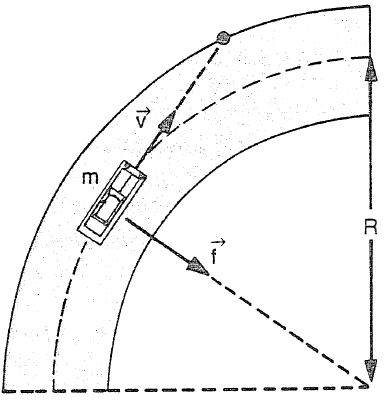
\includegraphics[scale=0.45]{figuras/fig_alvarenga_p222_31.png}
  \caption{Problema 5}
\end{figure}